\documentclass[12pt]{article}
\usepackage{graphicx}
\usepackage{amssymb, amsmath, amsthm, amssymb, amsthm}

\usepackage[usenames,dvipsnames]{color}
\usepackage{array}
\usepackage{relsize} 				%change equation font size
\usepackage{fancyref}
\usepackage{epsfig}
\usepackage{epstopdf}
\usepackage[center]{subfigure}
\usepackage{captcont} 			%break up figures with multiple subfigures
\usepackage{url} 					%format urls
\usepackage{setspace} 			%necessary? (from josh)
\DeclareGraphicsRule{.tif}{png}{.png}{`convert #1 `dirname #1`/`basename #1 .tif`.png}
%\usepackage[utopia]{math design}
\everymath{\displaystyle}
%--------------------------------------------------------------------------------------------------
% new commands
\newcommand\p{\partial}
\newcommand\kap{\kappa}
\newcommand\eps{\varepsilon}
\newcommand\la{\lambda} 
\newcommand\R{\mathbb{R}}
\newcommand\N{\mathbb{N}}
\newcommand\Z{\mathbb{Z}}
\providecommand{\abs}[1]{\lvert#1\rvert} 
\providecommand{\order}[1]{\operatorname{O}(#1)}
%---------------------------------------------------------------------------------------
% spacing and page setup
\textwidth = 6.4 in
\textheight = 9.2 in
\oddsidemargin = -0.0 in
\evensidemargin = -0.15 in
\topmargin = -0.1 in			 
\headheight = 0.0 in			
\headsep = 0.0 in
%\doublespacing
\parskip = 0.2in
\parindent = 0.0in
%\numberwithin{equation}{section}
\setcounter{page}{1} 				%number on first page
%========================================================
\begin{document}
%========================================================
%---title-------------------------------------------------------------------------------
%========================================================
\title{A global convergence conjecture \\for the FitzHugh-Nagumo system}
\author{Kelly M Paton, Eric N Cytrynbaum}
\date{\small{last edited: \today \space{} by KMP}}

\maketitle
%========================================================
%---abstract--------------------------------------------------------------------------
%========================================================
\abstract{

The FitzHugh-Nagumo system of partial differential equations (FHN) is a generic model for excitable media, often used to build a qualitative understanding of electrophysiological phenomena. A well-characterized traveling-pulse solution to FHN serves as a model for action potentials in cardiac tissue and other contexts. The stability of the traveling pulse has been well-studied but the more global problem of predicting when an arbitrary initial condition will converge to the uniform rest solution and when it will converge to the traveling pulse remains unsolved. Here, we prove the existence of an invariant winding number in an asymptotic limit of the FHN system called the singular FHN system (SFHN) that provides a crucial step toward a global convergence result. We provide evidence that our SFHN results extend with limitations to FHN as well and outline conditions under which the SFHN approximation fails. The invariant winding number provides explanations for several observations of physiological relevance. For example, it explains the requirements on stimulus protocols that allow the formation and elimination of reentrant rhythms in cardiac tissue.

Note: Michael's advice: submit to SIADS first; if rejected, IMA J App Math second (editor - Alan Champneys)

%========================================================
%---document------------------------------------------------------------------------
%========================================================

%========================================================
%---INTRODUCTION----------------------------------------------------------------
%========================================================

\section{Introduction}

The FitzHugh-Nagumo (FHN) system\footnote{We use the name FHN to refer to the generic model having a ``cubic-like'' nonlinearity rather than the specific model having precisely a cubic nonlinearity.} has long been used as a caricature-model for excitable media \cite{FH}. Despite its simplicity as a two variable system with a well developed theory describing many aspects of its dynamics, some behaviours of physiological importance are still poorly understood. For example, we know that there is a traveling pulse solution and understand its stability \cite{Fife1977} \cite{CytKeener2002} \cite{CKRT}. There is also a homogenous ``rest'' solution. However, predicting when an arbitrary initial condition will converge to one or the other of these is an unsolved problem. It has been conjectured that this convergence question for FHN with periodic boundary conditions (``FHN on a ring'') might reduce to a simple winding number condition in the phase plane \cite{GlassPersonal}. This topological conjecture has been examined numerically but inconclusively \cite{GlassPersonal}. 

The conjecture, should it be shown to hold, can be applied to a variety of situations.  For example, it offers a clear explanation of how a traveling pulse on a ring can be annihilated by a single point stimulus (as discussed in \cite{GJ1995}).  Conversely, it can be used to explain how a traveling pulse on a ring can be induced by an appropriate stimulus protocol. In a similar way, it relates to the mechanism proposed by Winfree for the generation of spiral waves in higher dimensions \cite{winfree-1980} \cite{WinfreeSA}. It also applies to explanations of the role of inhomogeneities of various space scales in the success and failure of cardiac defibrillation \cite{Keener2003} \cite{KeenerTop}.

In this paper, we turn to a useful reduction of the FHN system to shed light on the convergence conjecture. A separation of time and space scales in the FHN system allows for the use of asymptotic methods to derive a simpler related system of ODEs called the singular FitzHugh-Nagumo system (SFHN) \cite{ENC}. The convergence conjecture can be formulated for SFHN as well and the projection of the SFHN model into the phase plane has properties that make it more amenable to analysis. As a result, we are able to show the existence of an invariant winding number for the SFHN system that would seem to form the basis of a proof of the SFHN version of the convergence conjecture. Of course, results for the SFHN system do not always apply to the FHN system because the asymptotics break down, for example, around slowly-moving fronts and backs. However, for a large class of initial conditions, we present compelling numerical evidence that the long-term behaviour of FHN can also be predicted from the winding number of the initial condition. The global convergence conjecture for FHN includes a discussion on the allowable initial conditions, based on when FHN agrees with SFHN.

%It is generally believed that results for the singular FitzHugh-Nagumo (SFHN) system can be carried over to the $\eps \ne 0$ case in the FHN system by continuation arguments. However, our discussion revolves around the subtle structure of wave front behaviour near a stall point, a regime where this continuation argument breaks down.  Although we believe the results presented here can be useful to understanding convergence of the FHN system, we prefer to think of the SFHN system as a simple model of excitable tissue in its own right rather than as an approximation to the FHN system.

We begin by introducing the full and singular FHN system in Section \ref{sec:fhn}. In Section \ref{loop}, we define the phase-plane winding number, prove its invariance under SFHN dynamics and state a convergence conjecture for SFHN. In Section \ref{sec:ICs}, we explain how initial conditions for FHN can be converted into initial conditions for SFHN, thereby providing a means of predicting the behaviour of solutions to FHN for cases in which FHN solutions can be well-approximated by SFHN solutions. Applications of the conjecture are discussed in Section \ref{sec:applications}. In Section \ref{sec:invariance}, we prove the invariance of the winding number for SFHN. In Section \ref{sec:asympfailure}, we outline situations in which the initial conditions for FHN convert into initial conditions for SFHN that may lead to slow traveling fronts and backs. We expect these situations to violate or at least challenge the predictive power of the winding number.

%========================================================
%---EQUATIONS---------------------------------------
%========================================================

\section{The equations}\label{sec:fhn}
\subsection{The FitzHugh-Nagumo system}

The FitzHugh-Nagumo system consists of the equations
\begin{align}
\epsilon v_{\tau} &= \epsilon ^2 \frac{d^2v}{dx^2} + f(v,w), \label{FHNv}\\
w_{\tau} &= g(v,w)
\end{align}
where we have scaled time to the time constant of the recovery dynamics and the dimensional domain size is chosen so that the non-dimensional diffusion coefficient is $\epsilon^2$ where $\epsilon$ is the ratio of recovery to excitability time constants. The reaction term $f$ is a nonlinear cubic-like function in $v$ that is monotone decreasing in $w$. For fixed $w$ within some bistable interval $(w_{min}, w_{max})$ it has three zeros: $v_-(w)$, $v_0(w)$, and $v_+(w)$, the outer two of which correspond to stable steady states. The middle zero is unstable. Outside that bistable interval f has only a single zero. 

\begin{figure}
  \begin{center} 
    \includegraphics[scale=0.7]{eps/fhnvssfhnppp.eps} \caption{ \label{fig:ppp}
    {A traveling-pulse solution in the (a) FHN and (b) SFHN systems, shown in the spatial domain (left) and projected onto the parametric phase plane (right).}
    }
  \end{center} 
\end{figure} 

The function $g$ is chosen so that the system has a single spatially homogeneous stable solution at $(v,w)=(v_-(0),0)$. For the sake of calculation in Section \ref{sec:analysis}, we will take $g(v,w)=v-bw$ and $f(v,w) = H(v-a)-v-w$, with $a \in (0,1/2)$ and $b < a/(1-a)$ to ensure only one steady state. For all numerical calculations we set $a=0.1$ and $b=0.1$. For this $f$, $v_-(w)=-w$ and $v_+(w)=1-w$. There is technically no $v_0(w)$ curve due to the discontinuity in $f$, but $v_0(w)=a$ is a suitable replacement for our purposes. Other than the calculations in Section \ref{sec:analysis}, we continue to use the generic cubic-like $f$ for discussion of the conjecture.

\subsection{The singular FitzHugh-Nagumo system}

The singular FitzHugh-Nagumo (SFHN) system is derived by an asymptotic reduction of the FHN system (see \cite{ENC} for the full derivation).
First, in the limit of small epsilon, we can calculate the speed of a sharp transition layer as a function of the refractory variable $w$ at the transition \cite{MathPhys}:
\begin{equation}\label{speed}
c(w) = \sqrt{\frac{1-w-a}{w+a}}-\sqrt{\frac{w+a}{1-w-a}}
\end{equation}
where the sign convention is for a right-facing transition layer. Away from the transition, the outer solution collapses to the refractory ($v_-(w)$) and excited ($v_+(w)$) branches. The full state of the system can be defined by the locations of the transition layers, $\phi_i(\tau)$, and the $w(x,\tau)$ value on intervals between those layers. The evolution of these state variables is determined by the following equations:
\begin{align}
  w_\tau(x,\tau) & =  \left\{\begin{array}{lll}
    v_-(w)-\gamma w & & x \in (\phi_i,\phi_{i+1}),\ i \mbox{ even} \\ [0.3cm]
    v_+(w)-\gamma w & & x \in (\phi_i,\phi_{i+1}),\ i \mbox{ odd}
\end{array} \label{reduced_flow4} \right.\\
  \phi_i'(\tau)  & =  (-1)^{i} c(w(\phi_i,\tau)). \label{reduced_flow42}
\end{align}
where $\gamma=1+b<{1}/{(1-a)}$. A left-facing transition layer is indexed by odd $i$; right-facing transition layers have $i$ even. The factor of $(-1)^{i+1}$ in \eqref{reduced_flow42} ensures layer speeds are assigned the appropriate sign, where $c>0$ ($c<0$) corresponds to a right-moving (left-moving) transition layer. A transition layer at $w=1/2 -a$ formally has a traveling speed of $0$, even though the asymptotics break down here; we refer to this value of $w$ as $w_{\text{crit}}$, and call the layer a zero-speed layer. For our numerical calculations we take $\gamma = 1.1$ and $a=0.1$, which match the values we use for FHN calculations. 

When $w$ is low at a left-facing transition layer, the layer will move left, and we call it a front. When $w$ is high at a left-facing transition layer, the layer will move right, and we call it a back. In physiological terms, a front spreads excitation, while a back corresponds to recovery from post-excitation refractoriness.

For a given initial condition (IC), the number of fronts can only decrease (by front-front collisions) but it is possible for additional backs to appear dynamically, always in pairs. For example, if an IC has no transition layers initially and all of space is on the upper branch, $v_+(w)$, $w$ values will rise everywhere until the $w$ value reaches the upper end of the branch at $w_{max}$ at some point $x_b$. Two backs will then appear at $x_b$ and propagate away from each other, leaving in their wake an interval in $x$ on the lower branch. This corresponds to regions of space falling off the upper branch and rapidly converging to the lower branch which in SFHN is considered to occur instantaneously.

An initial condition for SFHN is specified by $w(x,0)$ and $\phi_i(0)$ ($i=1\dots
2n$) where the latter specify the locations of transition layers and $n$
is the number of excited intervals. Here, we focus on ``(S)FHN on a ring''. For FHN, this means periodic boundary conditions (BC) for equation \eqref{FHNv}. For SFHN, this means $\phi=0$ and $\phi=1$ are identified.

%========================================================
%---CONVERGENCE CONJECTURE----------------------------------------------
%========================================================
\section{Convergence in SFHN}\label{loop}

The state of the SFHN system on a ring can be
represented in the phase plane of the associated ODE as a closed curve
parameterized by $x$.  The closed curve takes the form of $2n$ horizontal line
segments (the transition layers) connected by curves along the upper and
lower branches of the $v$ nullcline.  This simplified representation
is referred to as the parametric phase plane, where the parameterization is in $x$. The conjecture is formulated primarily in terms of the shape of the IC in the phase plane.

We define the {\it zero speed line segment}, $\ell_0$, as the
horizontal line segment in the phase plane extending from the lower branch to the upper branch of the $v$ nullcline at the level $w=w_{\text{crit}}$ (see Figure \ref{fig_zero_line}). Note that zero-speed transition layers lie directly on this line segment. A {\it stall point} at time $\tau$ is any value of $x$ for which $w(x,\tau)=w_{\text{crit}}$. There need not be a transition layer at a stall point, but when there is, it is a zero-speed layer.\\

\begin{figure} %EDIT THE l to be ell
  \begin{center} 
    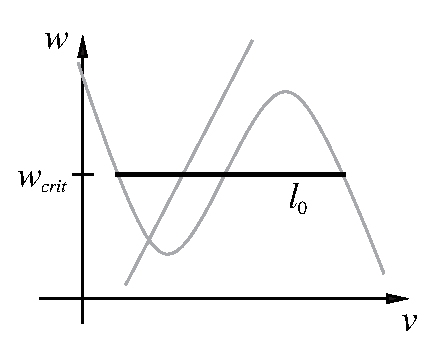
\includegraphics{eps/zero_line.eps} \caption{ \label{fig_zero_line}
    {The solid line through the middle of the phase plane,
    $\ell_0$, corresponds to a transition layer with zero speed.}}
  \end{center} 
\end{figure} 

\noindent {\bf Theorem: An invariant winding number for SFHN}\\
For the evolution of SFHN starting from any IC, fronts remain fronts, backs remain backs, and fronts cannot collide with backs. There is the possibility that backs collide with backs, fronts with fronts, and pairs of backs appear, but the winding number about $\ell_0$ in the parametric phase plane remains constant over time. Transition layers cannot slow down to zero speed.

\noindent {\bf Conjecture: Convergence to traveling pulses for SFHN}\\
If the SFHN traveling pulse is stable (see \cite{CytKeener2002} for stability conditions), then any IC converges to $m$ evenly spaced traveling pulses, where $m$ is the winding number of the initial condition around $\ell_0$ in the parametric phase plane. If the winding number is zero, the solution converges to the rest state. 
We do not address this convergence question here, but include its statement to emphasize the theoretical role of Part 1. \\\\Figure \ref{fig:SFHNloops} shows examples.

\begin{figure} %label \ell_0
  \begin{center} 
    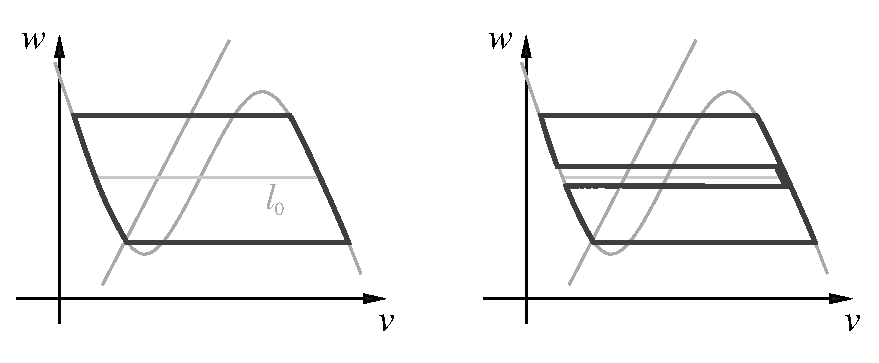
\includegraphics[scale=0.9]{eps/loop_ex2-01.eps} \caption{ \label{fig:SFHNloops}
    {Examples of initial conditions in the parametric phase
    plane. If the initial condition is admissible then it converges to (a) the traveling pulse
    for the initial condition on the left (winding number 1), and (b) rest
    for the initial condition on the right (winding number 0).}}
  \end{center} 
\end{figure}

\noindent {\bf Proof: An invariant winding number}

Suppose we have an initial condition for SFHN with two layers, one a right-facing front at $\phi_1(0)=f_0$ and the other a left-facing back at $\phi_2(0)=b_0$. Furthermore, suppose $w(x,0)=w_0(x)$ is a differentiable function everywhere on the ring. In front of the front and up until the initial position of the back ($b_0$), the system is in the unexcited/refractory state so the evolution of $w$ follows the lower branch dynamics. Thus, $w(x,t)$ decays to zero in time for each $x$ in that interval: $w(x,t)=w_0(x)e^{-\gamma t}$.

Suppose the front is moving toward the nearest stall point in front of it at $x_s(t)$. The velocity of the front is given by $c(w(\phi_1(t),t)$ and the velocity of the stall point can be found as follows. A stall point at time $t$ is defined as a point $x_s(t)$ at which $c(w(x_s(t),t)) = 0$. This occurs precisely when $w(x_s(t),t) = w_{crit}$. Taking derivatives of both sides with respect to $t$, we find that $$x_s'(t) = \frac{\gamma w_0(x_s(t))}{w_0'(x_s(t))}.$$

We proceed by contradiction beginning with the assumption that the front moves with a positive velocity until stalling at some time $t_s$. At $t_s$, we have that $\phi�(t_s)=0$. Looking at the expression for $x_s'(t)$ above, we seek to show that all terms in that expression are positive when $t=t_s$. First, note that $w(x_s(t_s),t_s)=w_0(x_s(t_s))e^{-\gamma t_s}=w_{crit}$ where the first equality follows from the solution $w(x,t)$ above and the second follows from the fact that $w$ is always $w_{crit}$ at a stall point. That means $w_0(x_s(t_s))=w_{crit}e^{\gamma t_s}>0$. Is it possible that $w_0'(x_s(t_s))<0$? If so, we would have $w(x_s(t_s)-\delta,t)>w_{crit}$ for sufficiently small $\delta>0$ at $t=t_s$ and therefore shortly before as well. This means the front would have had to move rightward through a region in which $w(x,t)>w_{crit}$ which is impossible -- a stall point with a negative $w$ slope would have to be the second nearest stall point to the front. So we conclude that either  (i) $x_s'(t_s)>0$ or (ii) $w_0'(x_s(t))=0$.

First consider case (i). We started with $\phi(0)<x_s(0)$ and are now considering the case in which we have $\phi�(t_s)=0$ and $x_s'(t_s)>0$ when those curves first touch. This is impossible.

Next consider case (ii). If $w_0'(x_s(t))=0$, it should be clear to see that $\lim_{t\to t_s^-}x_s'(t)=+\infty$. Such a curve cannot contact $\phi_1(t)$ which starts below it and has a zero slope at $t_s$.

Similar and symmetric reasoning can be applied to the case of a back approaching a stall point.

Thus, fronts remain fronts and backs remain backs. 

{\bf QED.}

To illustrate invariance with a simple example, consider the case of an initial condition with two transition layers, one a left-facing back and the other a right-facing front. The front is a transition from $v_+(w)$ to $v_-(w)$ (from left to right in $x$) at a value of $w<w_{crit}$ and thus moving to the right. The back is a transition from $v_-(w)$ to $v_+(w)$ at a value of $w>w_{crit}$ and thus also moving to the right (see Figure \ref{fig:ppp}(b)). As per the proof above, the front cannot change into a back nor vice versa. In the parametric phase plane, this means that the horizontal line representing the front, which is initially below $\ell_0$, cannot rise above $\ell_0$ as the system evolves and the back, which is initially above $\ell_0$, cannot drop below $\ell_0$. Thus the winding number is invariant. In space, this means that the front and back move together, possibly at different speeds but always in the same direction. If the convergence conjecture holds, their respective speeds converge to the same value. In the next section, we explore the invariance of the winding number for FHN.

%========================================================
%---Invariance in FHN-----------------------------------------------------------
%========================================================
\section{An invariant winding number for FHN}\label{sec:FHNinvariance}

Given that we have established the existence of an invariant winding number for SFHN, the obvious followup question is whether this result carries over to FHN. In as much as SFHN dynamics provide a good approximation to FHN dynamics, we assume for now that the answer is yes and explore the issue more carefully in the next section (Section \ref{SFHNgood}). Here, we describe how to calculate the winding number for an initial condition for FHN and thereby predict the long term behaviour of the system. 

Figure \ref{fig_loop_ex} shows two initial conditions for FHN projected into the phase plane. To convert these FHN initial conditions into SFHN initial conditions, we need to determine where transition layers set up under the fast dynamics in the multiple-time-scale analysis. To leading order, the fast manifold delivers points $(v(x),w(x))$ to either the lower ($v_-(w)$) or upper ($v_+(w)$) branch. The choice is determined by where the initial coordinates of the point in the phase plane lie relative to the middle branch, $v_0(w)$. If a point lies above/left of the middle branch, the appropriate SFHN initial condition for that point lies at the same $w$ value and $v$ on the lower branch (unexcited/refractory). If a point lies below/right of the middle branch, the appropriate SFHN initial condition for that point lies at the same $w$ value and $v$ on the upper branch (excited). 

Looking at the first FHN initial condition in Figure \ref{fig_loop_ex} (top left panel), we see two points at which the IC crosses the middle branch (circled). The two $x$ coordinates at which the IC curve crosses the middle branch become the initial locations of transition layers for the SFHN dynamics. One crossing lies above the zero-speed line, $\ell_0$, and thus becomes a back. The other, lying below $\ell_0$, becomes a front. The winding number for the resulting SFHN initial condition is 1 (or possibly -1 depending on the orientation of the parametrization) and so we predict convergence to a traveling pulse. 

The second FHN initial condition in Figure \ref{fig_loop_ex} (bottom left panel) has four crossings, two converging to backs and two converging to fronts. Going around the loop, we see that the two fronts occur in succession followed by the two fronts. The winding number in this case is zero. Note that the winding number for FHN can be found by counting the signed number of rotations about the point in the phase plane at which $\ell_0$ crosses the middle branch.

Movies S1 and S2 in the Supplemental Material show the evolution of qualitatively similar initial conditions to those shown in Figure 4, top left and bottom left panels respectively.

\begin{figure}
  \begin{center} 
    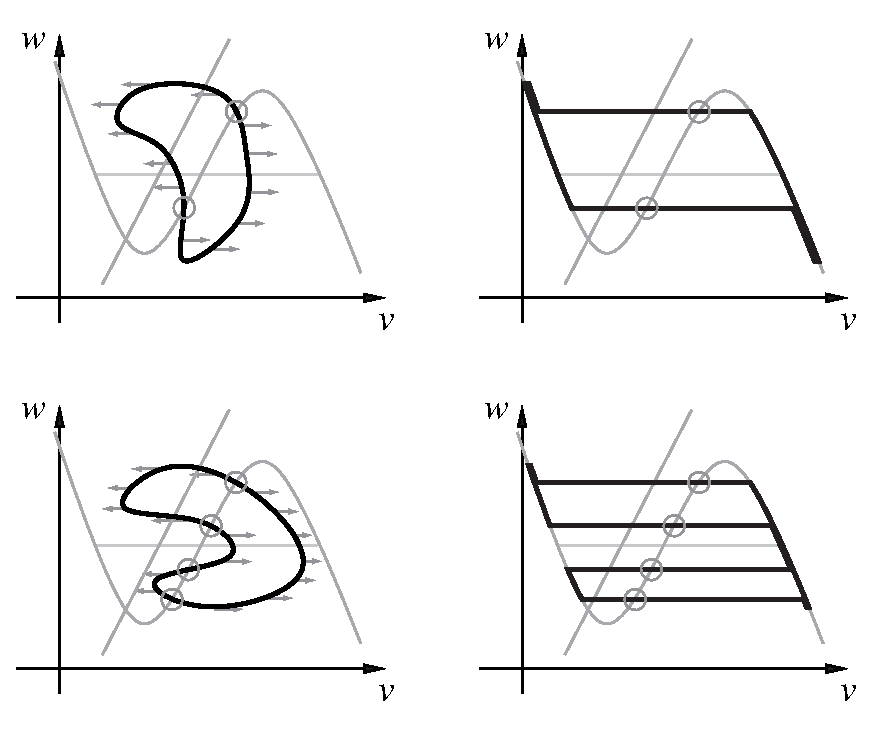
\includegraphics[scale=0.7]{eps/loop_ex.eps} \caption{ \label{fig_loop_ex}
    {
    Two FHN initial conditions in the parametric phase plane (left panels). SFHN initial conditions to which the FHN initial comditions in the left panel converge on the fast time scale in the singular limit (right panels). Transition layers appear wherever an initial condition crosses the middle branch of the cubic-shaped $v$ nullcline. Arrows show direction of movement in the phase plane.
}}
  \end{center} 
\end{figure}

\section{When is SFHN a good approximation of FHN?}\label{SFHNgood}

Say more intro here???

\subsection{Numerical comparison}
To demonstrate the extension to FHN, we performed numerical simulations of the FHN model on a ring for a family of ICs consisting of a front approaching an exponential refractory profile $w(x,0) = A e^{\lambda x}$. Although we found the GCT holds for any $A< w_{\text{crit}}$ and any $\lambda>0$ in SFHN, as predicted, the GCT does not hold at the edges of this region in FHN (see Figure \ref{fig:Alambda}). This is because steeper slopes allow a front to get close to zero speed, which is the region where SFHN and FHN diverge.

%=====figure======= 
\begin{figure}
\begin{centering}
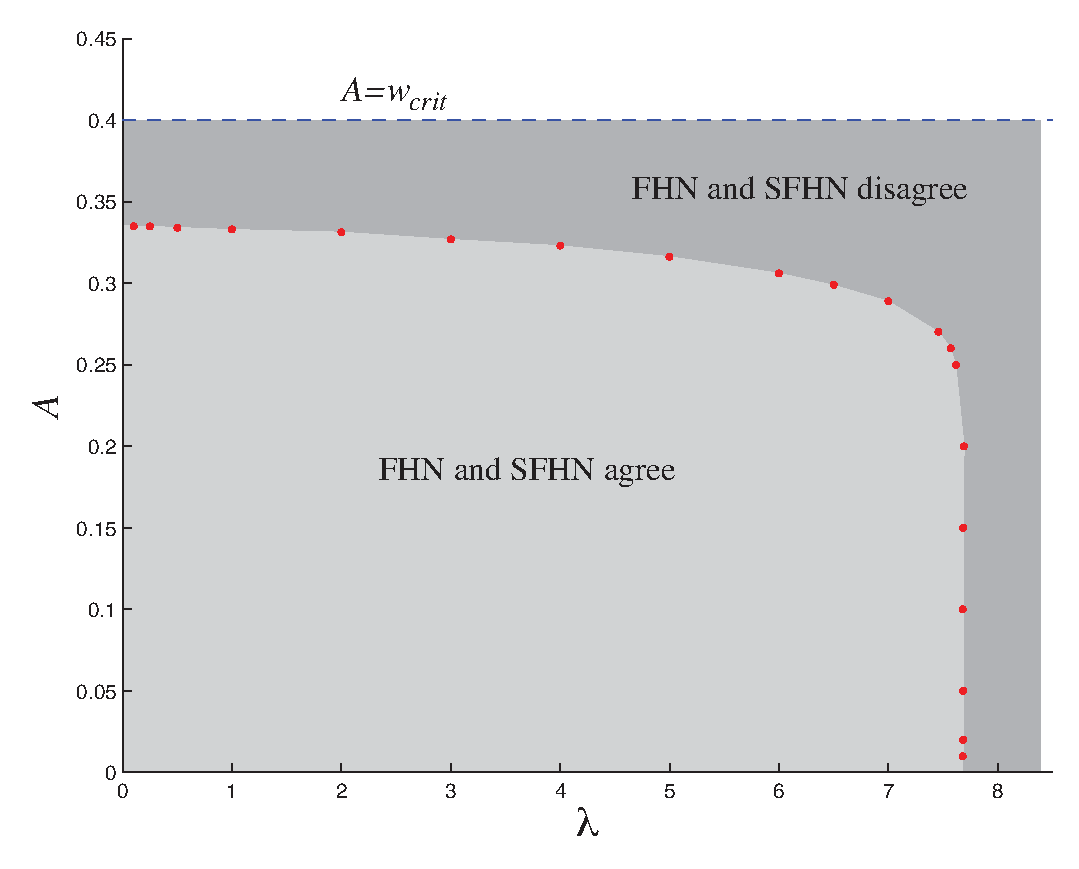
\includegraphics[width=5in]{eps/Alambda-simple-editedForPaper.eps}
\caption{{Traveling fronts in $v$ with $w(x,0)=A e^{\lambda x}$, $A<w_{\text{crit}}$, do not stall in SFHN. In much of the $A-\lambda$ plane, this is true for FHN as well, except when $A$ is close to $w_{\text{crit}}$ (meaning the layer starts close to a stall point) and for large $\lambda$. The dotted red curve marks the boundary between stalling and no stalling in FHN, and thus the boundary of ``admissible'' ICs of this type.}}\label{fig:Alambda}
\end{centering}
\end{figure}
%============== 


%========================================================
%---Kelly's exponential profile----------------------------------------------------------
%========================================================
\subsection{Wavefront with an exponential $w(x,0)$} \label{kelly}

An exponential $w(x,0)$ profile is an analytically tractable case that we can use to demonstrate the SFHN GCT: a front remains a front for this entire family of initial conditions.

Suppose $w(x,0)=A e^{\lambda x}$, with $A<w_{\text{crit}}$ and $\lambda>0$. Solving (\ref{reduced_flow4}) on the lower branch with this as an initial condition gives
\begin{equation}\label{w_exp}
 w(x,\tau)=Ae^{\lambda x-\gamma\tau}.
 \end{equation}
Set $w(x_s,\tau)=w_{\text{crit}}$ and solve for the position of the stall
point, 
$$x_s(\tau)=\frac{\gamma\tau}{\lambda} + \frac{1}{\lambda}\ln{\frac{w_{\text{crit}}}{A}},$$  
so that the speed of the stall point is given by 
\begin{equation}\label{eq:xs'}x_s'(\tau)=\frac{\gamma}{\lambda}.\end{equation}
The stall point moves to the right with constant speed that is inversely proportional to $\lambda$. How does the front behave with increasing $\lambda$? Here we calculate the distance between the front and the stall point as a function of $\lambda$ over time, and show that the interaction between the front and the stall point is qualitatively different for steep slopes versus mellow slopes.

\begin{figure}
  \begin{center} 
    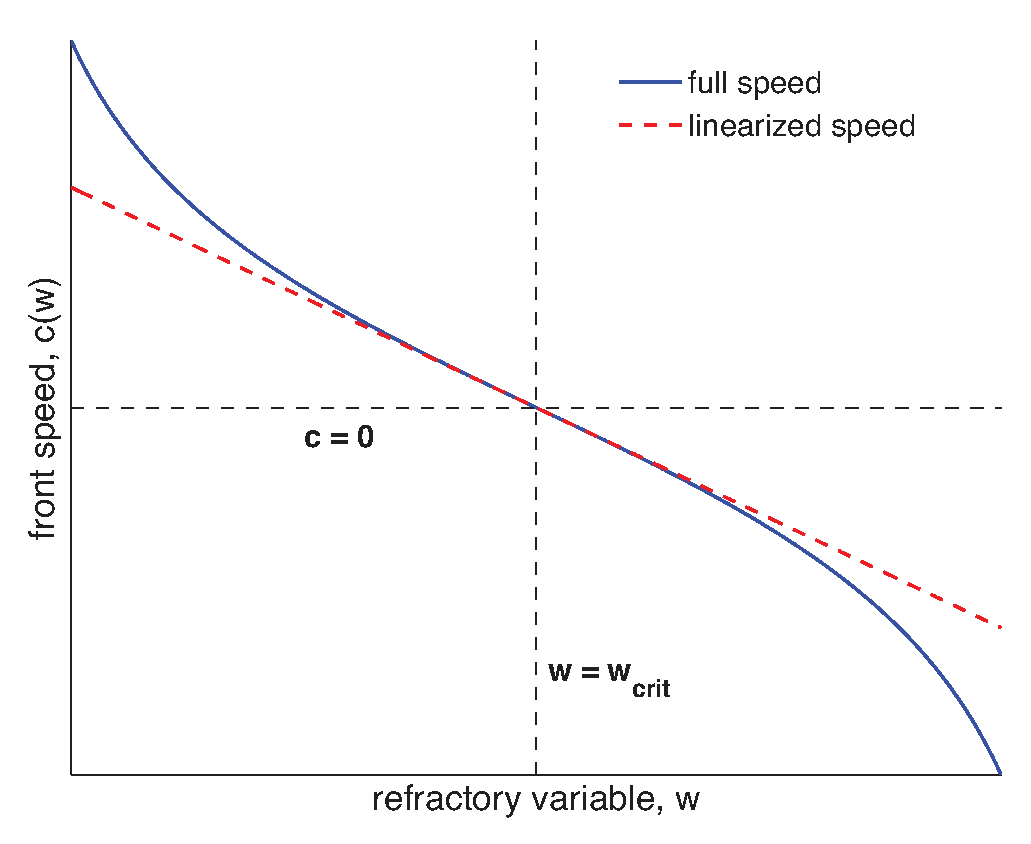
\includegraphics[scale=0.6]{eps/speedcomp_forPaper.eps} \caption{ \label{fig:speeds}
    {The full speed $c(w)$ from \eqref{speed} (solid curve, blue) which gives the speed of a right-facing layer, compared to its linearization (dashed curve, red) around $w=w_{\text{crit}}$.}}
  \end{center} 
\end{figure}

We are interested in the interaction between the front and the stall point, so we assume that they are close enough to each other that it is appropriate to approximate the front speed from (\ref{reduced_flow42}) with its linearization around $w=w_{\text{crit}}$ (see Figure \ref{fig:speeds}): 
\begin{align}\notag
\phi'(\tau) &= c(w(\phi(\tau),\tau)) \\
&\approx c(w_{\text{crit}}) + c_w(w_{\text{crit}}) \cdot\left(w(\phi(\tau),\tau)-w_{\text{crit}}\right).
\end{align}
With $c(w)$ from \eqref{speed} and dropping the approximation notation, this becomes 
\begin{equation}
  \phi'(\tau)= -4 \cdot (w(\phi(\tau),\tau)-w_{\text{crit}}). \label{lin_phi_eq}
\end{equation}
With $w(\phi,\tau)$ given by \eqref{w_exp}:
\begin{equation}
  \phi'(\tau)= - 4A e^{\lambda \phi - \gamma\tau} + 4w_{\text{crit}}.
\end{equation}
We solve this ODE to get
\begin{equation}
\phi (\tau)= -\frac{1}{\lambda}\ln{\left(\frac{4A}{4w_{\text{crit}} - \frac{\gamma}{\lambda}}\left(e^{\lambda(4w_{\text{crit}} - \frac{\gamma}{\lambda})\tau} - 1\right) + 1\right)} + 4w_{\text{crit}}\tau.
\end{equation}
The distance $d(\tau) = x_s(\tau)-\phi(\tau)$ can be written as
\begin{equation}\label{eq:d}
d(\tau) = \frac{1}{\lambda}\ln\left(\frac{1}{1-\frac{\gamma}{4w_{\text{crit}}\lambda}}\left(1-e^{(\gamma-4\lambda w_{\text{crit}})\tau}\right)+\frac{w_{\text{crit}}}{A}e^{(\gamma-4w_{\text{crit}}\lambda)\tau}\right)
\end{equation}
We verify that $d(\tau)$ is positive. We define parameters $\delta$ and $\alpha$:
\begin{align}
\delta = \frac{w_{\text{crit}}}{A} -1, \\
\alpha = \frac{\lambda}{\gamma/4w_{\text{crit}}} -1.
\end{align}
The restrictions on $A<w_{\text{crit}}$ and $\lambda>0$ tell us that $\delta>0$ and $\alpha>-1$. Note that  the nondimensional $\alpha$ replaces the dimensional $\lambda$ as a control on the steepness of the profile.

Analysis of \eqref{eq:d} in terms of $\delta$ and $\alpha$ reveals two distinct regions, separated by the boundary case of $\lambda =\gamma/4w_{\text{crit}}$ (or $\alpha= 0$). The resulting $d(\tau)$ expressions are
\begin{align}
d(\tau) = \left\{
\begin{array}{ll}
\frac{4 w_{\text{crit}}}{(1-\abs{\alpha})\gamma}\ln\left(1 +\frac{1}{\abs{\alpha}}\left(e^{\abs{\alpha} \gamma \tau}-1\right) + \delta e^{\abs{\alpha} \gamma \tau} \right), & 0>\alpha>-1\\
\frac{4 w_{\text{crit}}}{\gamma}\ln\left(1 +\delta + \gamma\tau \right), & \alpha = 0\\
 \frac{4 w_{\text{crit}}}{(1+\alpha)\gamma}\ln\left(1 + \frac{1}{\alpha}\left(1-e^{-\alpha \gamma \tau}\right) + \delta e^{-\alpha \gamma \tau} \right), & \alpha>0
\end{array}
 \right.
\end{align}
In all three cases, the arguments of the logarithm functions are greater than $1$ for all $\tau, \delta>0$ and $0<\gamma<1/1-a$, ensuring that $d(\tau)>0$ for any choice of $\lambda$ and $A$, an observation which supports the GCT.

We gain further insight into the behaviour in each parameter region by looking at the speed of the front in the limit of large $\tau$:
\begin{align}
\lim _{\tau \to \infty} \phi'(\tau) = \left\{
\begin{array}{ll}
4w_{\text{crit}}, & 0>\alpha>-1\\
\gamma/\lambda, & \alpha>0
\end{array}\right.
\end{align}
Comparing these front speeds to the stall point speed $x_s' = \gamma/\lambda$ \eqref{eq:xs'} is illuminating. For \mbox{${0>\alpha>-1}$}, corresponding to small $\lambda<\gamma/4w_{\text{crit}}$ or mellow profiles, the front asymptotically approaches a constant speed of $4w_{\text{crit}}$, which is slower than the stall point speed. The stall point thus escapes the front, always moving further away. For $\alpha>0$, or large $\lambda$ and steep profiles, the front speed asymptotes to a constant value that matches the stall point speed. The front and the stall point move forward at a fixed separation. The qualitative propagation behaviour in each region is depicted in Figure \ref{fig:sfront}.

%===figure=====
\begin{figure}
\begin{centering}
{\subfigure[{\bf $\lambda>\gamma/4w_{\text{crit}}$}]{\includegraphics[width=4in]{eps/frontbig_sFHN_editedForPaper.eps}}}\\
{\subfigure[{\bf $\lambda<\gamma/4w_{\text{crit}}$}]{\includegraphics[width=4in]{eps/frontsmall_sFHN_editedForPaper.eps}}}
\caption[Sample front and stall point behaviour for wavefronts facing exponential refractory profiles.]{{\bf Sample front and stall point behaviour for wavefronts facing exponential refractory profiles.}  The position of the front, $\phi$ (solid blue line), and stall point $x_s$ (dashed red line) over time for the singular FHN system. The upper panel in (a) displays fixed-distance propagation behaviour for steep profiles, $\lambda>\gamma/4w_{\text{crit}}$ or $\alpha>0$.  The lower panel in (b) displays divergent behaviour for mellow profiles, $\lambda<\gamma/4w_{\text{crit}}$ or $0>\alpha>-1$.}\label{fig:sfront}
\end{centering}
\end{figure}
%==============  

This result illustrates the sometimes counterintuitive nature of the theorem due to the coupled effect of $w$ on wave speed and stall point speed.



%========================================================
%---Eric's wavefront passage-------------------------------------------------------
%========================================================
\subsection{Dynamically steepening slopes}\label{slopes}

Here we explore ways in which slopes can steepen during the evolution of solutions, and thus create the opportunity for a front to get close enough to zero speed for FHN to behave differently from SFHN. This cannot happen in between transition layers, but layers themselves can generate steep slopes. For example, suppose a wave back moving from left to right is located just ahead of a stall point on a positive slope in $w(x,\tau)$. While the back is moving slowly, the $w$ values in front are rising and the $w$ values in back are falling, steepening the positive slope. If the back manages to avoid stalling, it can nonetheless leave behind a potential stall zone for any wave front that might follow (see Figure \ref{fig_steep_w}). Any initial condition that can lead to a steep enough slope to stall a FHN front is categorized as ``inadmissible'' under the GCC.

%===figure=====
\begin{figure}
  \begin{center} 
    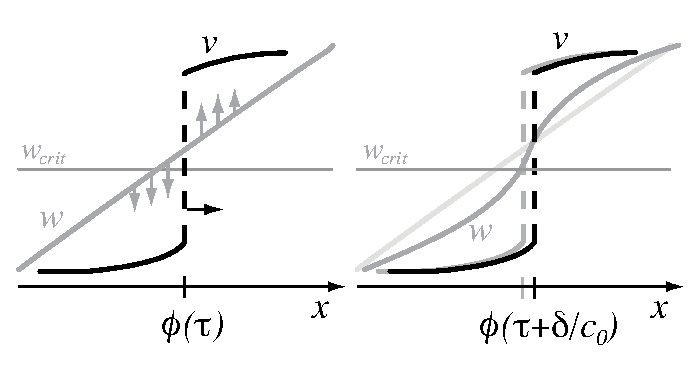
\includegraphics{eps/steep_w.eps} \caption{ \label{fig_steep_w}
    {A schematic example of how a wave back can generate a
    potential zero-speed zone for a wave front in FHN. Left panel: A wave back at $\phi(\tau)$ sits just ahead of a stall point. Grey arrows show the dynamics of $w$. Right panel: The same wave back shortly after. Note $w(x,t)$ has developed a steeper slope. The plot from the left panel is replicated in light grey for comparison. A wave front coming in from the left could interact with this steep w zone and approach a zero speed even though the initial condition did not have a steep slope in $w$ itself.}}
  \end{center} 
\end{figure} 
%============== 

We can formalize this scenario by calculating the relationship between the slope at a point just before a back moves through and just after. Let $\phi(0)=0$ and $w(0,0)=w_0$. We assume that $w_0>w_{\text{crit}}$ (the layer is a back) and its orientation is such that $\phi'(0)>0$. We consider a small interval $0<x<\delta$ in front of the wave back. We assume that $w$ is linear in this interval and that the speed of the front is constant:

\begin{figure}% need to include vertical v axis and label v+ and v- branches
  \begin{center} 
    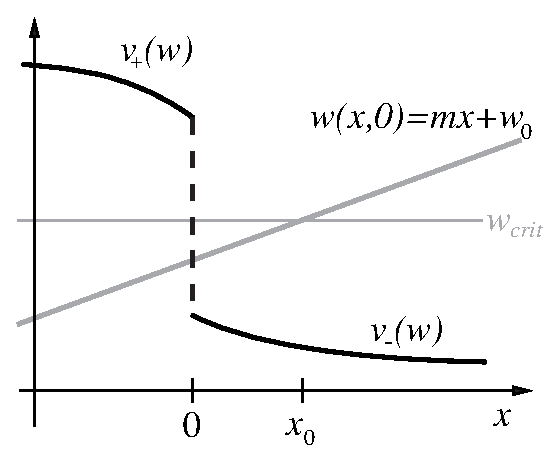
\includegraphics[scale=0.7]{eps/stall.eps} \caption{ \label{fig_stall}
    {The initial condition of a locally linear $w$ near a front.}}
  \end{center} 
\end{figure}

\[ w(x,0) = mx+w_0  \ \ \ \mbox{for} \ \ 0 < x < \delta, \]
\[ \phi'(\tau) = c_0 >0 \ \ \ \mbox{for} \ \ 0<\tau<\frac{\delta}{c_0}. \]
so that  \[\phi(x/c_0) = x.\]
At each point $x$ between $0$ and $\delta$, the passage of the back forces the dynamics to switch from the upper branch to the lower branch. At one point $x$, the wave spends $x/c_0$ units of time on the upper branch and $(\delta - x)/c_0$ units of time on the lower branch. Thus, 
\begin{equation}\label{eq:w_delta}
w\left(x, \frac{\delta}{c_0}\right) = \left[\frac{1}{\gamma} - \left(\frac{1}{\gamma} - mx - w_0 \right) e^{-\gamma x/c_0}\right] e^{-\gamma(\delta-x)/c_0}
\end{equation}
for $0<x<\delta$. To find the slope immediately after the back has passed, we calculate:
\[\lim_{\delta \to 0} w_x\left(0,\frac{\delta}{c_0}\right) = m + \frac{1}{c_0}.\]
Thus, a point $x$ on the ring with a slope given by $w_x(x, \tau^-)=m$ immediately preceding the passage of a wave back will have a slope given by $w_x(x, \tau^+)=m + 1/c_0$ immediately after the wave back passes. For backs close to stall points, $c_0$ is small and the change in slope as the back passes a point can thus be large. This discontinuity in $w_x$ is the result of the discontinuity in the $w$ dynamics generated by the switch from the upper to the lower branch.

A similar calculation gives the relationship between the slope before and after the passage of a wave front:
% not verified, but makes sense. gamma shouldn't play a role here either.
\[\lim_{\delta \to 0} w_x\left(0,\frac{\delta}{c_0}\right)=m-\frac{1}{c_0}.\]

In each case, the passage of the transition layer generates a steeper slope that could potentially slow down a transition layer (of the opposite orientation) following it. This possibility of longer-range interaction emphasizes the need for caution in applying a merely local condition on admissibility.


%========================================================
%---APPLICATIONS-----------------------------------------------------------
%========================================================
\section{Applications}\label{sec:applications}
\subsection{Background}

The applications of the GCT that we focus on here relate to pathological rhythms in excitable media, in particular, simple forms of reentry in cardiac tissue. Normal cardiac signaling is driven by the SA node, an oscillatory pace maker near the top of the heart. However, self-sustained rhythms that consist of a pulse of excitation traveling through cardiac tissue along a closed loop can arise in various ways (e.g. tachycardia associated with Wolff-Parkinson-White syndrome or atrial flutter). Such rhythms are themselves problematic for the patient but also introduce the risk of more serious forms of reentry (e.g. atrial or ventricular fibrillation). In this section we consider (S)FHN as a model for reentry and, in particular, look at mechanisms by which reentry can be introduced and eliminated. 

Introducing reentry to a ring of excitable media in a uniform rest state requires some kind of stimulus protocol. Mathematically, this appears as a short-lived non-autonomous forcing term $I_{app}(x,t)$ added to the $v$ equation. The stimulus drives the state of the system from rest to a traveling pulse. Eliminating reentry is accomplished using a stimulus protocol that accomplishes the reverse. With the GCT in mind, we characterize these transitions as changing the winding number of the solution, from 0 to 1 (or -1) in the former case and 1 (or -1) to 0 in the latter case. Note that the GCT is applied to the state of the system immediately following the stimulus protocol, treating that moment as an IC for subsequent evolution.

\subsection{Inducing reentry}

The introduction of reentry to a system that is at the spatially
uniform rest state requires an asymmetrical stimulus protocol.  Figure
\ref{fig_reentry} shows a schematic representation of the S1-S2
stimulus protocol required to generate a pulse on a ring.  The first
stimulus, S1, generates two symmetric pulses moving in opposite
directions. If the S2a stimulus in panel (b) is given a sufficiently
large (positive) amplitude, a loop is created by excitation of an
interval in the middle of the resting phase. Once S2a terminates, the GCT can be applied to the state of the system (thought of as an initial condition) indicating that the solution converges to the traveling pulse.
Alternately, the S2b stimulus in panel (b), given a sufficiently large
(negative) amplitude, creates a loop around $\ell_0$, the zero speed line,
by de-excitation of an interval in the middle of the excited phase.

%===figure====== 
\begin{figure}
  \begin{center} 
    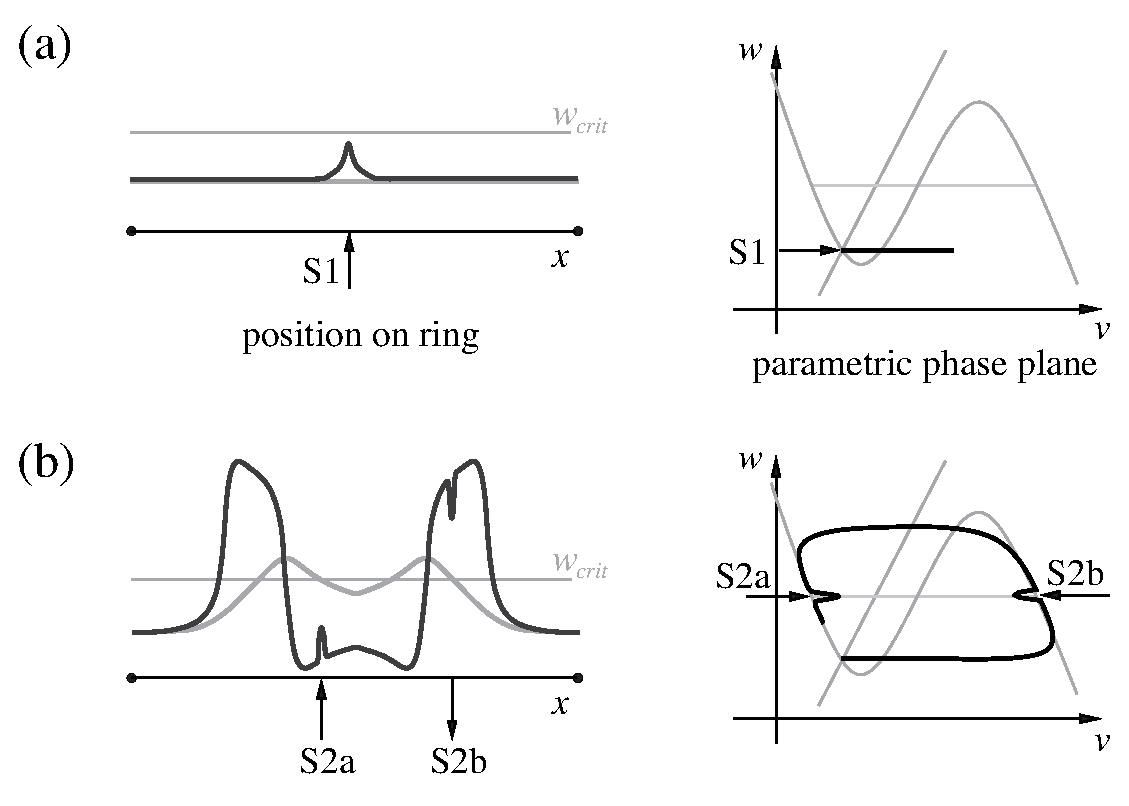
\includegraphics[scale=0.75]{eps/reentry.eps} \caption{ \label{fig_reentry} {The S1-S2 stimulus protocol required to induce reentry.
    (a) An S1 stimulus generates two traveling pulses.  (b) The S2a
    stimulus creates a loop around the zero speed line by
    excitation.  (c) The S2b stimulus creates a loop
    around the zero speed line by de-excitation.  Arrows indicate
    location and polarity of stimuli.  Solid curves on the left are
    $v(x)$ and dashed curves are $w(x)$.  The dotted line is at
    $w=w_{crit}$.  The transition layers in these figures were drawn
    as steep but not discontinuous for clarity of presentation -- layers should actually be discontinuities.}}
  \end{center}
\end{figure}
%============== 

\subsection{Eliminating reentry}

A similar stimulus protocol can be used to annihilate a reentrant
rhythm.  Glass and Josephson \cite{GJ1995} demonstrate numerically
(for the FHN system) that a properly timed and properly located point stimulus
can annihilate a traveling pulse. The requirement of appropriate
timing and location can be explained in terms of the zero speed line.

Figure \ref{fig_annihilate} shows two appropriate stimulus protocols for successfully annihilating a traveling pulse. An annihilating stimulus, A1 or A2, must remove the loop around the zero speed line. Furthermore the $w$ profile in the traveling pulse must not have steep slopes in the vicinity of the newly formed transition layers, in keeping with admissibility.

%====figure======= 
\begin{figure}
  \begin{center} 
    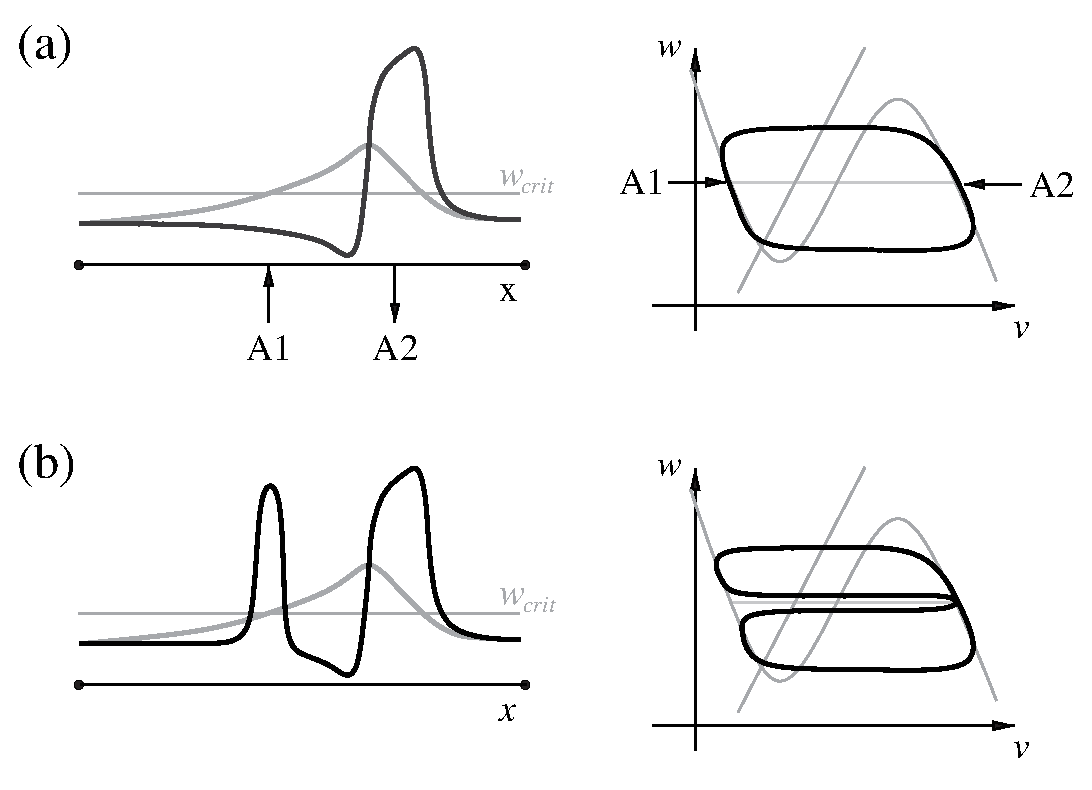
\includegraphics[scale=0.75]{eps/annihilate.eps}\caption{
    \label{fig_annihilate}{(a) Two possible annihilating stimuli, A1 and A2, are both capable of
    eliminating the loop around the zero speed line.  (b) The outcome
    of a sufficient large amplitude A1 stimulus.}} 
  \end{center} 
\end{figure} 
%============== 

\subsection[Defibrillation and the space scale of inhomogeneities in
cardiac tissue]{Defibrillation and the space scale of \\ inhomogeneities in
cardiac tissue}

The application of large external electric fields to cardiac tissue
creates virtual transmembrane electrodes throughout the tissue.  The
exact mechanism by which these virtual electrodes (VE) appear is a
matter of much debate \cite{dosdall2010} but it is generally accepted that
inhomogeneities in tissue structure, primarily variations in the
conductivity tensor, are the source.  Using a bidomain model in one
spatial dimension, Keener derives an expression for the VE amplitude
that depends on the amplitude of the external stimulus and the
gradient of the conductance \cite{Keener1996}.

Using an averaging technique in the limit of inhomogeneities of a small spatial scale, Keener explains the dependence of defibrillation on the amplitude of the stimulus and the independence of defibrillation from the timing of the stimulus, consistent with clinical and experimental observations.

For tissue with inhomogeneities of a large spatial scale only, the
averaging technique is not valid and another approach to predicting the response of the system to a stimulus is needed.  The
GCT offers an answer.  Because of the space scale of
inhomogeneity being considered, the generated VE pattern has
essentially the same effect as a small number of point stimuli applied
at various locations on the ring (see Figure \ref{fig_defib}).

%====figure======= 
\begin{figure}
  \begin{center} 
    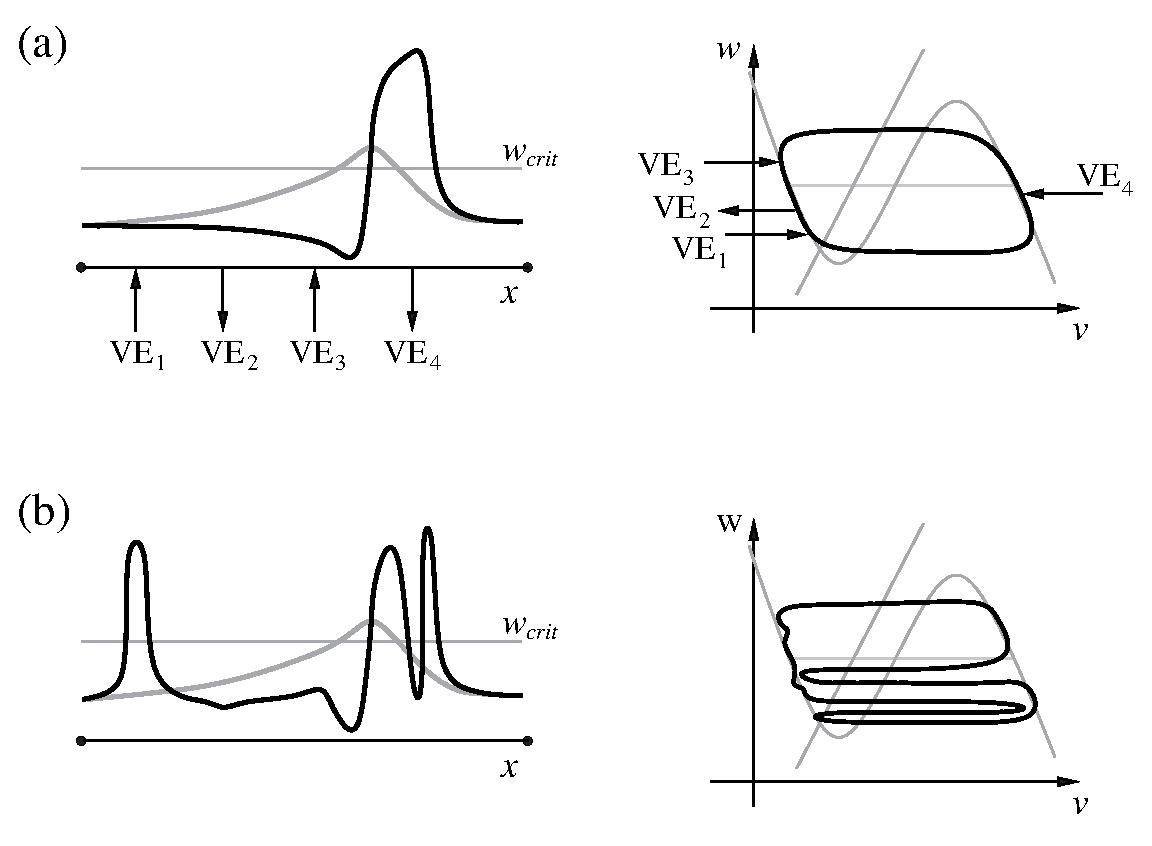
\includegraphics[scale=0.75]{eps/defib.eps} \caption{ \label{fig_defib}
    {An unsuccessful attempt to annihilate a traveling pulse.
    Panel (a) shows the positions of four virtual electrodes (VE), two
    depolarizing and two hyperpolarizing before the stimulus is
    applied.  Panel (b) shows the poststimulus effect of the VEs.
    $\mbox{VE}_1$ and $\mbox{VE}_4$ are successful at depolarizing and
    hyperpolarizing, respectively, the tissue in their immediate
    vicinity.  $\mbox{VE}_2$ and $\mbox{VE}_3$ have negligible impact.
    The loop around the zero speed line is not removed by the
    stimulus.  However, had the stimulus been applied moments later,
    $\mbox{VE}_4$ would have been applied at a slightly different
    location on the traveling pulse leading to a successful
    removal of the loop and annihilation of the traveling pulse. Note the possibility of reversing the direction of travel of the pulse if, for example, VE3 and VE4 both succeed in changing the winding number about $\ell_0$ for a net change of -2.
    }}
  \end{center} 
\end{figure} 
%============== 

Figure \ref{fig_defib} shows a case in which a stimulus applied at the moment shown would not lead to annihilation. However, a stimulus moments later would allow VE4 to change the winding number to 0. Similarly, a stimulus moments earlier would allow VE3 to change the winding number to 0. Thus, even for sufficiently large amplitude stimuli, defibrillation is not independent of timing when relying on inhomogeneities of a large space scale.
A numerical demonstration of these claims for FHN can be found in
\cite{Keener2003}.



%========================================================
%---CONCLUSIONS----------------------------------------------------------
%========================================================
\section{Conclusions}

The GCT states that we can predict propagation behaviour in the SFHN system based entirely on the phase plane representation of the initial condition. When extending the GCT to a global convergence conjecture for FHN, certain initial conditions can be dismissed as inadmissible if a transition layer is too close to the zero-speed layer. We find that ``closeness'' is modulated by the steepness of $w(x,0)$, which is information that is not visible in the parametric phase plane.

%We also note that these results are based on analysis near the zero-speed regime, and thus should not be blindly extended to the full FHN system. A suggestion for future work is the development of a modified SFHN system that better emulates the behaviour of the FHN system near stall points.  This may involve finding the $\order{\epsilon}$ correction term to the leading-order wave speed, a problem which would involve a solvability condition with adjoint eigenfunctions. Ideally, the expansion of the wave speed to a two term approximation would be sufficient to increase the accuracy of the singular system without sacrificing its simplicity.  However, the inner-layer recovery dynamics become more complicated for small speeds, which means the singular description may become more complicated than the current two ODEs.  In either case, an improvement to singular approximation near the zero-speed regime would be a useful addition to the FHN toolbox. Until such an improvement is found, we encourage the use of the SFHN system as a model in its own right -- with the modified loop conjecture as a method of predicting its convergence -- and note that caution must be used when using it to predict convergence in the full FHN system.

\appendix

\bibliographystyle{plain}
\bibliography{sfhnpaper.bib}

\end{document}